\documentclass{bredelebeamer}

\begin{document}

\title[INFO-F-412 - Traffic Light Control]{\textbf{Traffic Light Control} \\INFO-F-412 -- Formal Verification} % The short title appears at the bottom of every slide, the full title is only on the title page

\author[]{Jamal \textsc{Ben Azouze}, Marien \textsc{Bourguignon}, Nicolas \textsc{De Groote}, \\Simon \textsc{Picard}, Arnaud \textsc{Rosette}, Gabriel \textsc{Ekanga}}
\institute[ULB] % Your institution as it will appear on the bottom of every slide, may be shorthand to save space
{
Université Libre de Burxelles \\ % Your institution for the title page
\medskip
\textit{Département d'Informatique} % Your email address
}
\date{4 Juin 2015} % Date, can be changed to a custom date

\begin{frame}
\titlepage % Print the title page as the first slide
\end{frame}

\begin{frame}{Sommaire}
\tableofcontents % Throughout your presentation, if you choose to use \section{} and \subsection{} commands, these will automatically be printed on this slide as an overview of your presentation
\end{frame}

\section{Introduction}
\begin{frame}{Introduction}

\end{frame}

\section{Uppaal}
\begin{frame}{Uppaal}

\end{frame}

\section{Acteurs et automates}
\subsection{Acteurs de l'environnement}
\begin{frame}{bla}

\end{frame}

\subsection{Automates de l'environnement}
\begin{frame}{bla}

\end{frame}

\subsection{Contrôleur}
\begin{frame}{Contrôleur}

\end{frame}

\section{Model checking}
\subsection{Liveness properties}
\begin{frame}[fragile]{Liveness properties}

\begin{block}{1. A pedestrian will never wait indefinitely to cross the road}
\begin{verbatim}
p --> q = A[] (p imply A<> q)

PedestrianGeneratorEast.PushButton --> PedestrianGeneratorEast.Cross
\end{verbatim}
\end{block}

\begin{block}{2. A car will never wait indefinitely to enter the crossroad}
\begin{verbatim}
(CarGeneratorEast.AcceptCar&&queueIndex[E]!=0) -->
        CarGeneratorEast.CarCrossing
(CarGeneratorSouth.AcceptCar&&queueIndex[S]!=0) -->
        CarGeneratorSouth.CarCrossing
(CarGeneratorWest.AcceptCar&&queueIndex[W]!=0) -->
        CarGeneratorWest.CarCrossing
\end{verbatim}
\end{block}

\begin{block}{3.No deadlock}
\begin{verbatim}
A[] not deadlock
\end{verbatim}
\end{block}

\end{frame}

\subsection{Safety properties}
\begin{frame}[fragile]{Safety properties}
\begin{block}{1. The pedestrian light will never be green at a wrong time}
\begin{verbatim}
A[] not
(pedestrianLight == GREEN &&
    (carLight[E] == GREEN ||
        (carLight[W] == GREEN && queue[W][0] == U) ||
        (carLight[S] == GREEN && queue[S][0] == R)
    )
)
\end{verbatim}
\end{block}

\begin{block}{2. No pedestrian will be hit by a car}
\begin{verbatim}
A[] not
(PedestrianGeneratorEast.Cross &&
    (CarGeneratorEast.CarCrossing ||
        CarGeneratorWest.CarCrossing && queue[W][0] == U ||
        CarGeneratorSouth.CarCrossing && queue[S][0] == R
    )
)
\end{verbatim}
\end{block}
\end{frame}

\begin{frame}[fragile]{Safety properties}
\centering
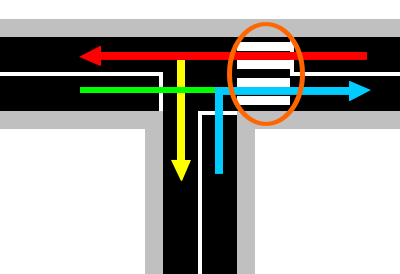
\includegraphics[scale=0.8]{images/pietonCollision.png}

\end{frame}


\begin{frame}[fragile]{Safety properties}

\begin{block}{3. Cars should never collide}
\begin{verbatim}
A[] not (
(
    CarGeneratorWest.CarCrossing && queue[W][0] == U && 
    ((
        CarGeneratorEast.CarCrossing && queue[E][0] == L
    ) || (
        CarGeneratorSouth.CarCrossing && 
        ( queue[S][0] == L || queue[S][0] == R )
    ))
) || (
    CarGeneratorWest.CarCrossing && queue[W][0] == R 
    && CarGeneratorEast.CarCrossing && queue[E][0] == L
))
\end{verbatim}

Same idea for the two other orientations.
\end{block}

\end{frame}
\begin{frame}[fragile]{Safety properties}
\centering
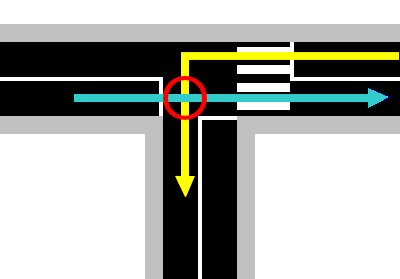
\includegraphics[scale=0.8]{images/exempleCollision.png}

\end{frame}

\begin{frame}[fragile]{Safety properties}
\begin{block}{4. No combination of light allowing car collision}
\begin{verbatim}
A[] not 
(
    (carLight[E] == GREEN && queue[E][0] == L &&
        (
            (carLight[S] == GREEN && queue[S][0] == L) ||
            (carLight[W] == GREEN &&
                (queue[W][0] == U || queue[W][0] == R)
            )
        )
    ) || 
    (carLight[E] == GREEN && queue[E][0] == U &&
    carLight[S] == GREEN && queue[S][0] == L)
)
\end{verbatim}

Same idea for the two other orientations.
\end{block}
\end{frame}


\section{Conclusion}
\begin{frame}{Conclusion}

\end{frame}
\end{document}